%%%%%%%%%%%%%%%%%%%%%%%%%%%%%%%%%%%%%%%%%%%%%%%%%%%%%%%%%%%%%%%%%%%%%%%%
%     LaTeX source code to approximate a Draft NIST Technical report
%	  Instructions for authors: tinyurl.com/techpubsnist 
%	DOI watermark will be added on final PDF
% 	Developed by K. Miller, kmm5@nist.gov 
%	Last updated: 22-March-2019
%%%%%%%%%%%%%%%%%%%%%%%%%%%%%%%%%%%%%%%%%%%%%%%%%%%%%%%%%%%%%%%%%%%

%%%%%%%%%%%%%%%%%%%%%%
% Template further altered by Armen Amirkhanian
% for use with UA lab courses in an effort to 
% have a standardized format for lab documents
% Last update 9-April-2020
%
% TODO:
% --Get the appendices to dynamically link, tocloft causes problems
%%%%%%%%%%%%%%%%%%%%%%

\documentclass[12pt]{article}
\usepackage{amsmath}
\usepackage{amsfonts}   % if you want the fonts
\usepackage{amssymb}    % if you want extra symbols
\usepackage{graphicx}   % need for figures
\usepackage{xcolor}
\usepackage{bm}
\usepackage{secdot}		
\usepackage{mathptmx}
\usepackage{float}
\usepackage[utf8]{inputenc}
\usepackage{textcomp}
\usepackage[hang,flushmargin,bottom]{footmisc} % footnote format
\usepackage{xspace}
%\usepackage{lineno}
\usepackage{ragged2e}
\usepackage{parskip}
\usepackage{textcomp}
\usepackage{environ}
\usepackage{multirow}
\usepackage{textgreek}

\usepackage{tikz}
\usetikzlibrary{shapes.geometric, arrows}
\tikzstyle{startstop} = [rectangle, rounded corners, minimum width=2cm, minimum height=1cm,text centered, draw=black, fill=red!20]
\tikzstyle{arrow} = [thick,->,>=stealth]

\usepackage{titlesec}
\titleformat{\section}{\normalsize\bfseries}{\thesection.}{1em}{}	% required for heading numbering style
\titleformat*{\subsection}{\normalsize\bfseries}

\usepackage{tocloft}	% change typeset, titles, and format list of appendices/figures/tables
\renewcommand{\cftdot}{}	
\renewcommand{\contentsname}{Table of Contents}
\renewcommand{\cftpartleader}{\cftdotfill{\cftdotsep}} % for parts
\renewcommand{\cftsecleader}{\cftdotfill{\cftdotsep}}
\renewcommand\cftbeforesecskip{\setlength{4pt}{}}
\addtolength{\cftfignumwidth}{1em}
\renewcommand{\cftfigpresnum}{\figurename\ }
\addtolength{\cfttabnumwidth}{1em}
\renewcommand{\cfttabpresnum}{\tablename\ }
\setlength{\cfttabindent}{0in}    %% adjust as you like
\setlength{\cftfigindent}{0in} 

\usepackage{enumitem}         % to control spacing between bullets/numbered lists

\usepackage[numbers,sort&compress]{natbib} % format bibliography 
\renewcommand{\bibsection}{}
\setlength{\bibsep}{0.0pt}

\usepackage[hidelinks]{hyperref}
\hypersetup{
	colorlinks = true,
urlcolor ={blue},
citecolor = {.},
linkcolor = {.},
anchorcolor = {.},
filecolor = {.},
menucolor = {.},
runcolor = {.}
pdftitle={},
pdfsubject={},
pdfauthor={},
pdfkeywords={}
}
\urlstyle{same}

\NewEnviron{letter}{%
\begin{quote}
\fbox{%
\begin{minipage}{\linewidth}
\setlength{\parskip}{\baselineskip}
%\letterfont
\BODY
\end{minipage}
}
\end{quote}
}

\usepackage{epstopdf} % converting EPS figure files to PDF

\usepackage{fancyhdr, lastpage}	% formatting document, calculating number of pages, formatting headers
\setlength{\topmargin}{-0.5in}
\setlength{\headheight}{39pt}
\setlength{\oddsidemargin}{0.25in}
\setlength{\evensidemargin}{0.25in}
\setlength{\textwidth}{6.0in}
\setlength{\textheight}{8.5in}

\usepackage{caption} % required for Figure labels
\captionsetup{font=small,labelfont=bf,figurename=Fig.,labelsep=period,justification=raggedright} 

%%%%%%%%%%% !!!!!REQUIRED - FILL OUT METADATA HERE !!!!!!!! %%%%%%%%%%%%%%
%%%%%%%%%%%%%%%%%%%%%%%%%%%%%%%%%%%%%%%%%%%%%%%%%%%%%%%%%%%%%%%%%%%%%%%%%%
\newcommand{\CourseNum}{CE262}
\newcommand{\CourseName}{Civil Engineering Materials}
\newcommand{\LabTitle}{Aggregate Relative Density}
\newcommand{\LastUpdate}{Fall 2020}

%%%%%%%%%%%%%%%%%%%%%%%%%%%%%%%%%%%%%%%%%%%%%%%%%%%%%%%%%%%%%%%%%%%%
%   	BEGIN DOCUMENT 
%%%%%%%%%%%%%%%%%%%%%%%%%%%%%%%%%%%%%%%%%%%%%%%%%%%%%%%%%%%%%%%%%%%%
\begin{document}
	\urlstyle{rm} % Format style of \url   
%\linenumbers
\begin{titlepage}
\begin{flushright}
\LARGE{\textbf{\CourseNum{} -- \CourseName}}\\
\vfill
\Huge{\textbf{\LabTitle}}\\
    \vfill
%%%%%%%%%%%%%%%%%%%%%%%%%%%%%%%%%%%%%%%%%%%%%%%%%%%%%%%%%%%%%%%%%%%%
%	Authors - add complete list of authors, affiliations will be 
%   added on title page
%%%%%%%%%%%%%%%%%%%%%%%%%%%%%%%%%%%%%%%%%%%%%%%%%%%%%%%%%%%%%%%%%%%%
    \large Dr. Armen Amirkhanian, P.E.\\
\vfill
%%%%%%%%%%%%%%%%%%%%%%%%%%%%%%%%%%%%%%%%%%%%%%%%%%%%%%%%%%%%%%%%%%%%
%	The DOI is automated based on metadata.	
%%%%%%%%%%%%%%%%%%%%%%%%%%%%%%%%%%%%%%%%%%%%%%%%%%%%%%%%%%%%%%%%%%%%
\normalsize This work is licensed under the Creative Commons Attribution-ShareAlike 4.0 International License. To view a copy of this license, visit:
\href{http://creativecommons.org/licenses/by-sa/4.0/}{http://creativecommons.org/licenses/by-sa/4.0/}.


\includegraphics[width=0.07\textwidth]{cc.eps}
\includegraphics[width=0.07\textwidth]{by.eps}

\includegraphics[width=0.07\textwidth]{sa.eps}
\vfill

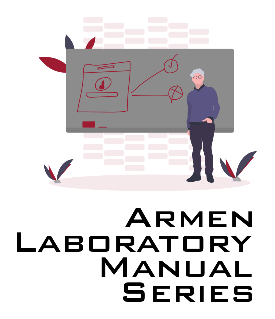
\includegraphics[width=0.3\linewidth]{Logo.eps}\\ 
 
  
\end{flushright}
\end{titlepage}

\begin{titlepage}
\begin{center}
\normalsize 
Certain commercial entities, equipment, or materials may be identified in this document in order to describe an experimental procedure or concept adequately. Such identification is not intended to imply recommendation or endorsement by The University of Alabama or the listed authors, nor is it intended to imply that the entities, materials, or equipment are necessarily the best available for the purpose.\\
\vfill
Any opinions or recommendations are solely those of the author(s) and do not represent the official view or policy of The University of Alabama.
\end{center}
\begin{flushright}
\vfill
\normalsize 
This document was last updated in \textbf{\LastUpdate} and should contain \textbf{\pageref{LastPage}} pages of content exclusive of these title pages, abstract, and other front matter. If the document appears to be incomplete, please contact the author(s).\\
\vfill
At that time the chief engineer was almost always the chief test pilot as well.\\That had the fortunate result of eliminating poor engineering early in aviation.\\
\textit{Igor Sikorsky}
\end{flushright}
\end{titlepage}
%%%%%%%%%%%%%%%%%%%%%%%%%%%%%%%%%%%%%%%%%%%%%%%%%%%%%%%%%%%%%%%%%%%%
%   Start front matter - page number starts with "i"
%%%%%%%%%%%%%%%%%%%%%%%%%%%%%%%%%%%%%%%%%%%%%%%%%%%%%%%%%%%%%%%%%%%%
\pagenumbering{roman}
\section*{Abstract}
\normalsize The specific gravity and absorption properties of an aggregate source are critical pieces of information to have so that durable concrete and asphalt mixture designs can be developed. While an aggregate can be at a variety of moisture contents ranging from oven-dry to dripping wet, we usually only need the specific gravities related to two moisture states: oven-dry and saturated surface-dry (SSD).

\vfill
\section*{Keywords}
\normalsize relative density; pycnometer; absorption.\\
\pagebreak
%%%%%%%%%%%%%%%%%%%%%%%%%%%%%%%%%%%%%%%%%%%%%%%%%%%%%%%%%%%%%%%%%%%%
%   Table of Contents is required
% 	List of Tables & Figures required if more than 5 tables/figures
%%%%%%%%%%%%%%%%%%%%%%%%%%%%%%%%%%%%%%%%%%%%%%%%%%%%%%%%%%%%%%%%%%%%
\begin{center}
\tableofcontents
\pagebreak
\listoftables
\listoffigures
\end{center}
\pagebreak
\section*{Required Specifications}
The following specifications are required to complete this laboratory exercise:
\begin{description}
\item[ASTM C127] Standard Test Method for Relative Density (Specific Gravity) and Absorption of Coarse Aggregate
\item[ASTM C128] Standard Test Method for Relative Density (Specific Gravity) and Absorption of Fine Aggregate
\end{description}

The following specifications are optional, but they are listed here in the event more information is needed to complete the laboratory exercise:
\begin{description}
\item[ASTM C125] Terminology Relating to Concrete and Concrete Aggregates
\item[ASTM D6026] Standard Practice for Using Significant Digits in Geotechnical Data
\end{description}
\pagebreak
%%%%%%%%%%%%%%%%%%%%%%%%%%%%%%%%%%%%%%%%%%%%%%%%%%%%%%%%%%%%%%%%%%%%
%   Start body of text - page number starts with "1"
%%%%%%%%%%%%%%%%%%%%%%%%%%%%%%%%%%%%%%%%%%%%%%%%%%%%%%%%%%%%%%%%%%%%
\section{Fine Aggregates}
\label{sec:intro}
\pagenumbering{arabic}
\normalsize 
There are several definitions for what constitutes a fine aggregate. A geotechnical application may consider fine aggregate to be anything between a \#4 sieve and the \#200 sieve while an asphalt concrete application may consider fine aggregate to be anything between the 9.5 mm and \#200 sieves. A fine aggregate is defined by ASTM C125 as:

\begin{letter}
(1) aggregate passing the 9.5-mm (3/8-in.) sieve and almost entirely passing the 4.75-mm (No. 4) sieve and predominantly retained on the 75-\textmu m (No. 200) sieve; or (2) that portion of an aggregate passing the 4.75-mm (No. 4) sieve and retained on the 75-\textmu m (No. 200) sieve
\end{letter}

We will use this definition for our laboratory exercise. Another confusing part about fine aggregate characterization is the use of the terms ``specific gravity'' and ``density'' and ``unit weight''. The naming conventions that are used for civil engineering aggregates in ASTM specifications is shown in Table \ref{tab:ASTMname} along with their deprecated terms\footnote{Deprecated means the term is actively being discouraged from use but you may still come across it in older documentation.}. Specifically for the fine aggregate laboratory exercise, we will use the terminology and procedures outlined in ASTM C128.

\begin{table}[h]
\centering
\caption{Current terminology used in ASTM standards with respect to densities of aggregates.}
\label{tab:ASTMname}
\begin{tabular}{ccc}
\hline
Current Term & Deprecated Term & Units \\ \hline
Relative Density & Specific Gravity & -- \\
Bulk Density & Unit Weight & lbs/ft$^3$ or kg/m$^3$ \\ \hline
\end{tabular}
\end{table}

\newpage
\subsection{Objectives}
\label{ssec:headingscap}
At the completion of this lab exercise section, you will have satisfied the following objectives:
\begin{enumerate}
    \item Perform saturated-surface-dry (SSD) relative density measurement on a fine aggregate
    \item Prepare fine aggregate sample for oven-dry relative density measurement
    \item Perform calculations necessary to determine the relative density properties of a fine aggregate
    \item Perform calculations necessary to determine the absorption capacity of a fine aggregate
\end{enumerate}

\subsection{Learning Outcomes}
At the completion of this lab exercise, you should be able to:
\begin{itemize}
    \item understand what saturated-surface-dry and oven-dry conditions are for a fine aggregate
    \item perform calculations necessary to characterize the relative density and absorption capacity of a fine aggregate
    \item understand the appropriate range of possible values for relative density and absorption capacity for fine aggregates
    \item present calculated values in a useful and professional manner
\end{itemize}

\pagebreak
\subsection{Procedure}
The fine aggregate characterization procedure is divided into three parts: preparation, execution, and analysis. Given the importance placed on weight (mass) measurements, it is critical to keep detailed notes and follow steps carefully and accurately. There are a number of measurements that will be taken and it is easy to get the values mixed up. It may even help you to take a picture of the scale with the material on it for each step so you have a visual record of the weight and what was actually weighed.

This exercise can take some time due to the fact you have to carefully dry the aggregate to a precise state (i.e. SSD). Patience is key. If the sample gets too dry, your results will be ``wrong''. Very generally, you will slowly dry a completely saturated fine aggregate sample until the surface just begins to dry but the porosity of the sample is filled with water. You will then take a series of mass measurements to determine both the mass and volume of the sample. Finally, you will oven dry the sample to determine how much water it took to fill the porosity just to the surface. A schematic of the different moisture states is shown in Fig. \ref{fig:moisturestates}.

\begin{figure}[H]
    \centering
    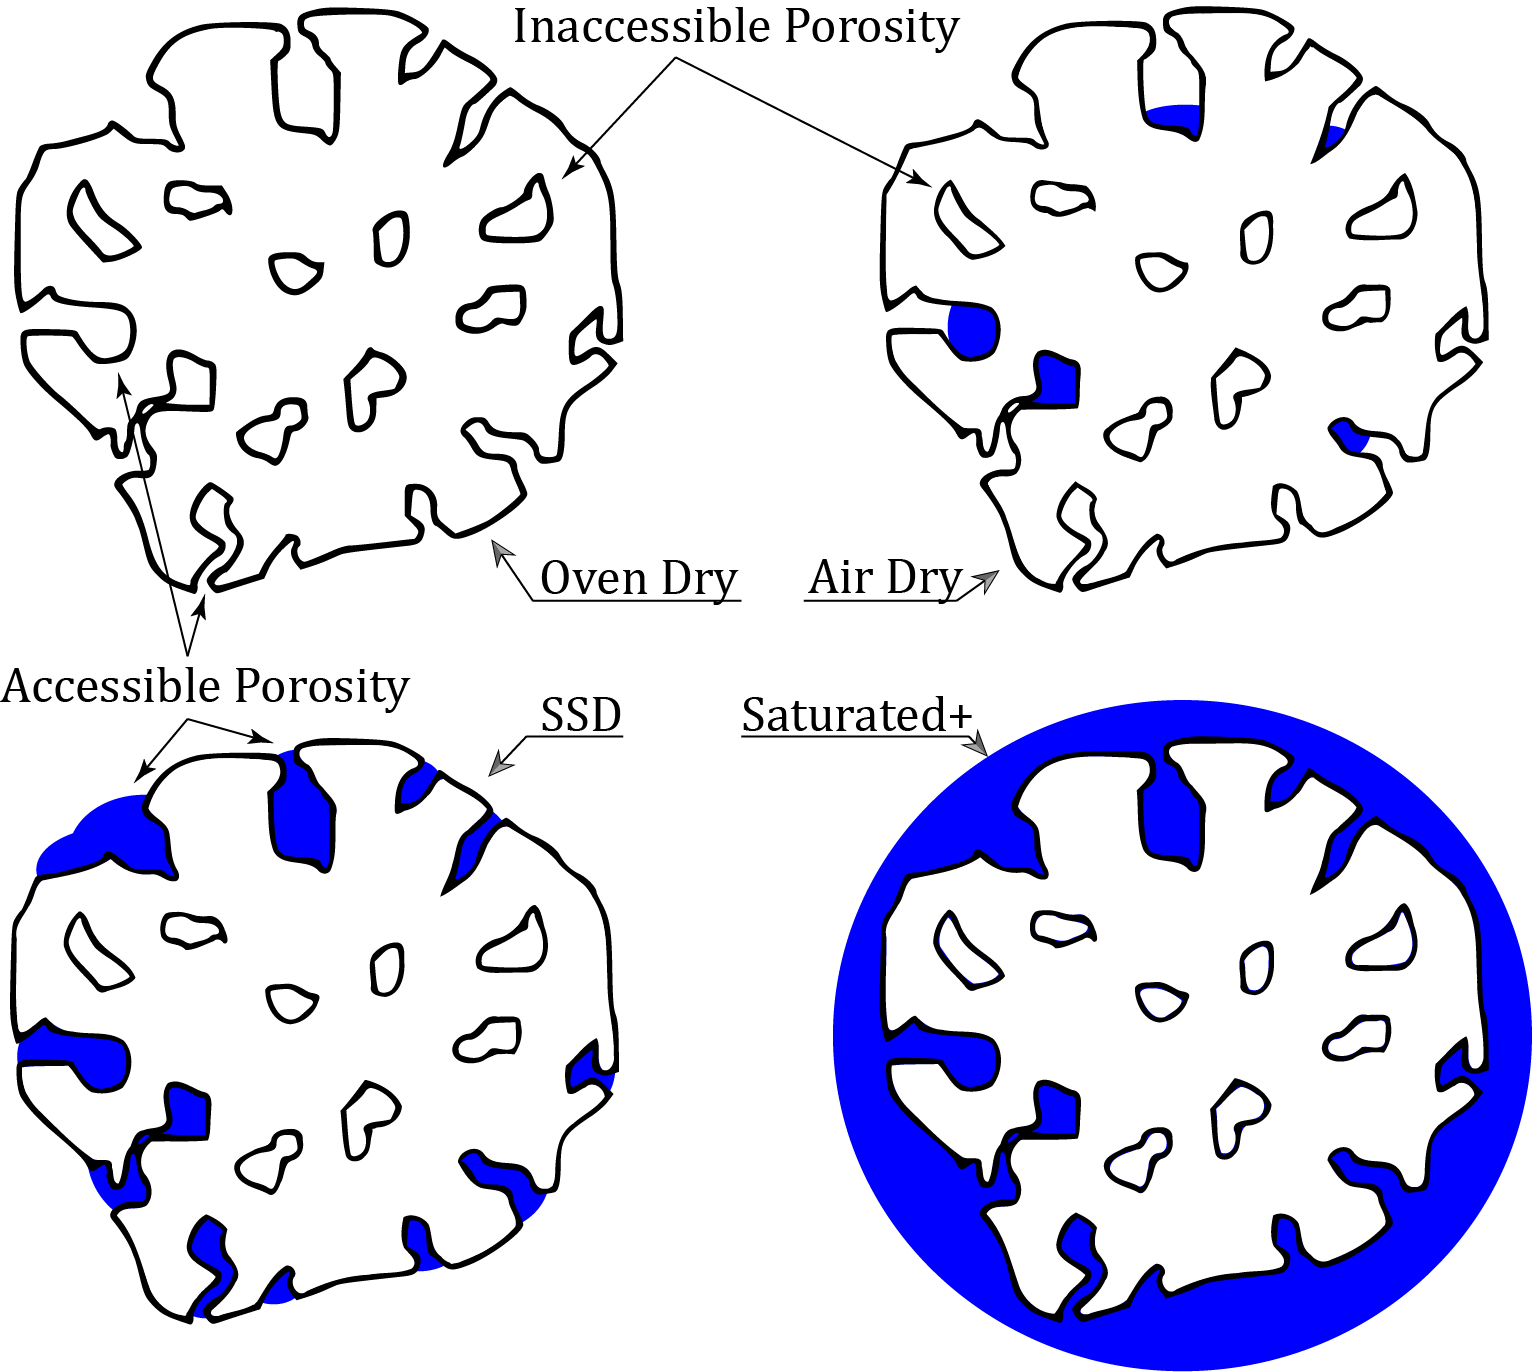
\includegraphics[width=0.6\textwidth]{Moisture_States_Schematic.png}
    \caption{Examples of different moisture states that can be present in aggregate. The shaded blue portions indicate water. The air dry and saturated+ states are arbitrary (e.g. air dry just means it is between oven-dry and saturated-surface-dry).}
    \label{fig:moisturestates}
\end{figure}

\subsubsection{Preparation}
For the fine aggregate characterization, you will need your saturated sample and a device called a pycnometer. Well, it is not a true pycnometer because we are going to ignore the required thermometer and other geometric requirements. Let's be real, it a jar (Fig. \ref{fig:jar}) that previously had some sort of food (probably pickles) in it and a glass plate (Fig. \ref{fig:glassplate}). Because of the magnitude of the measurements we are doing, using any rigid container will work as a pycnometer for our purposes.

\begin{figure}[H]
    \centering
    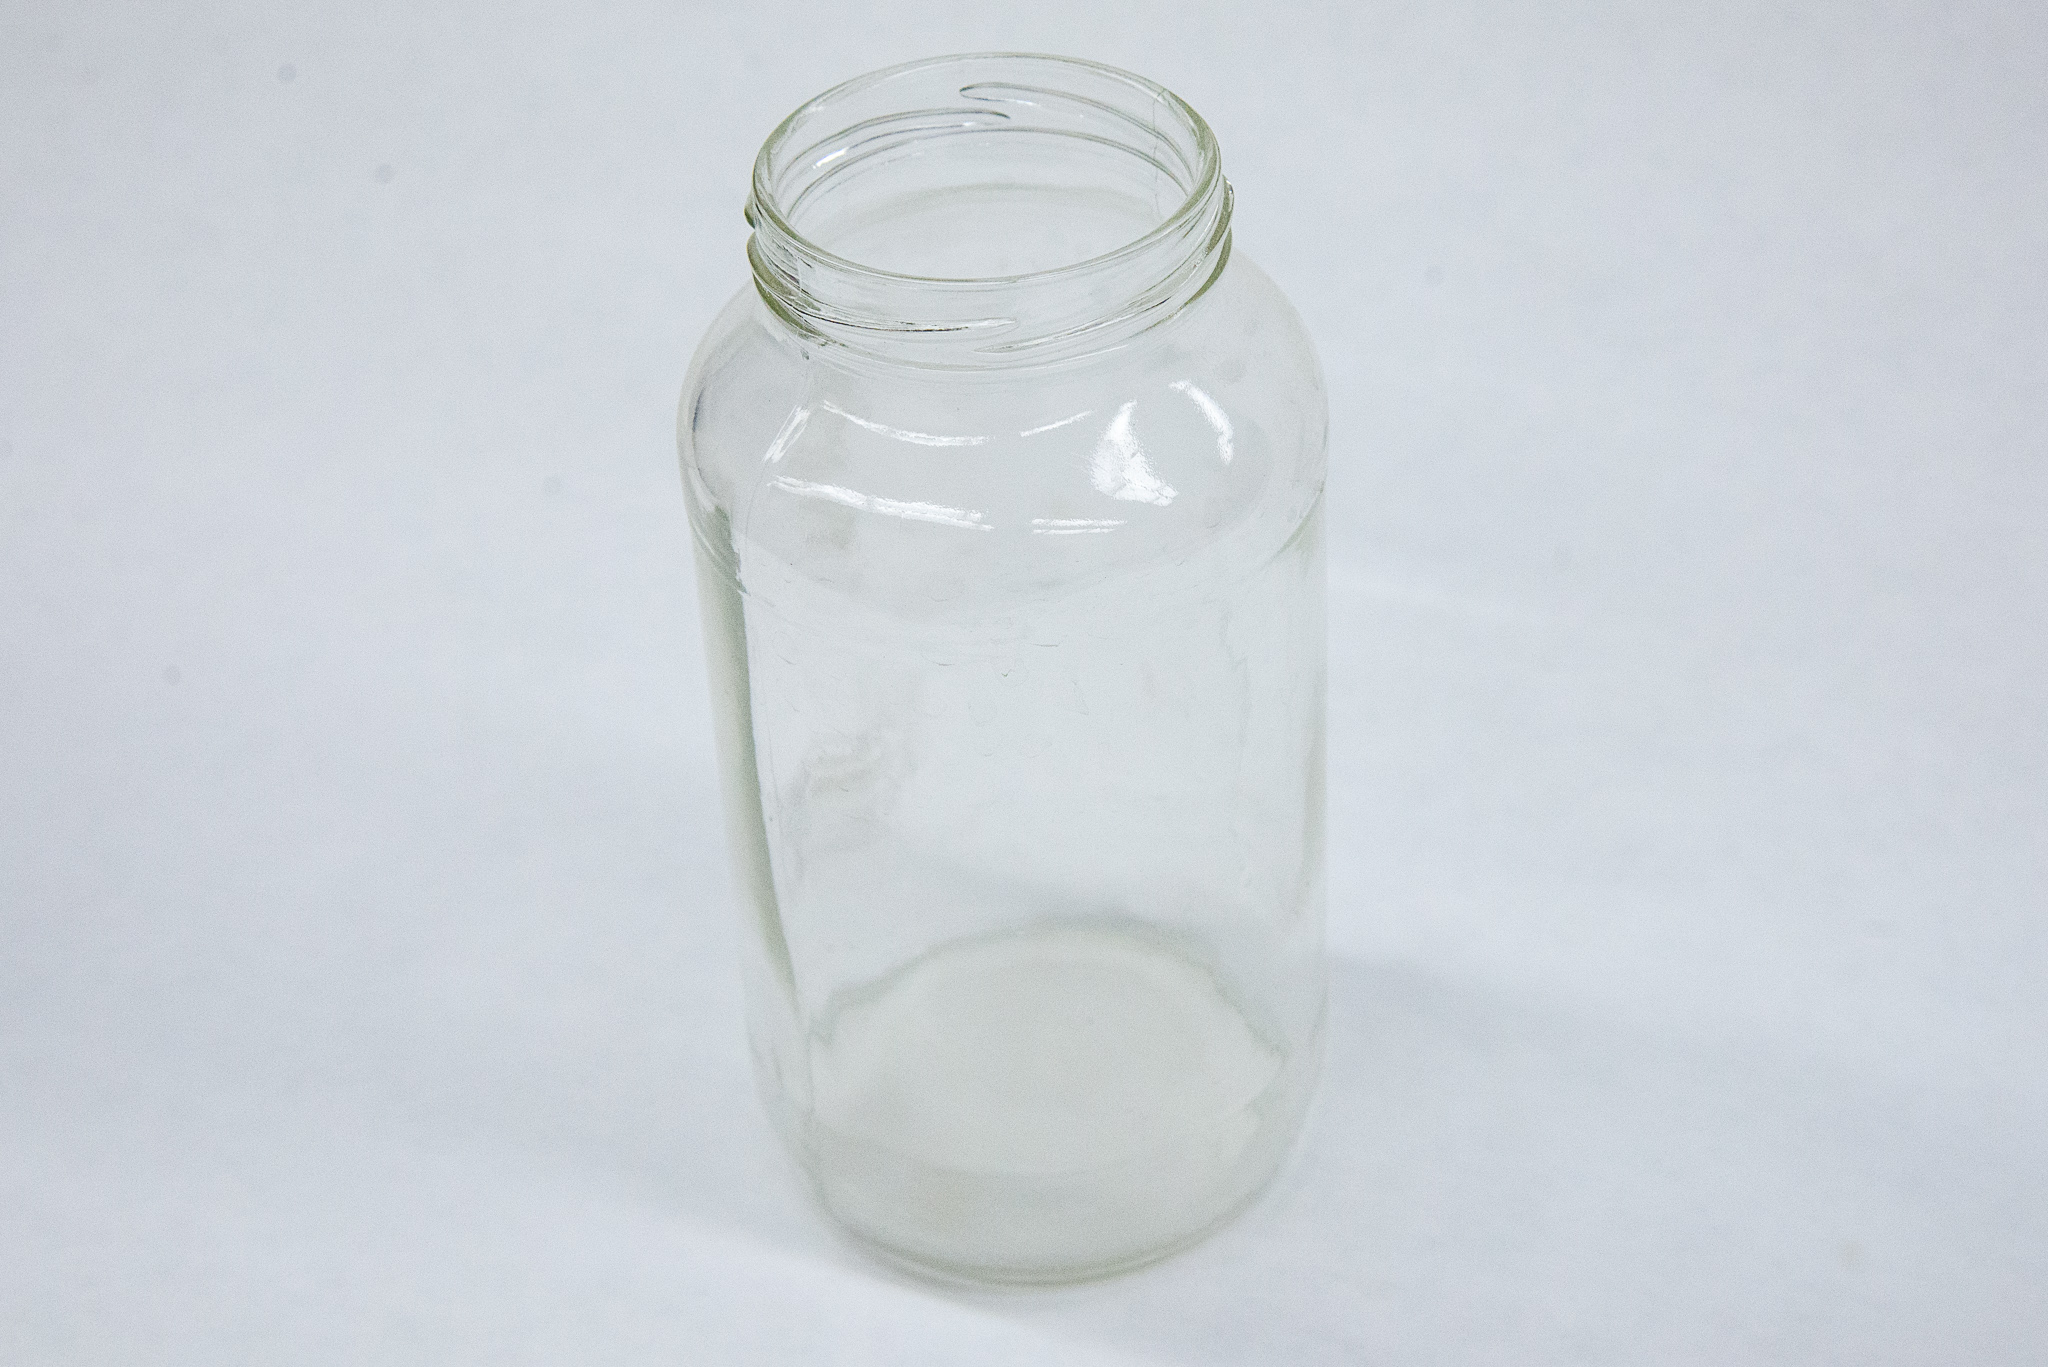
\includegraphics[width=0.7\textwidth]{GEO_5850.jpg}
    \caption{Example of the type of jar that might be used for the fine aggregate measurements.}
    \label{fig:jar}
\end{figure}

\begin{figure}[H]
    \centering
    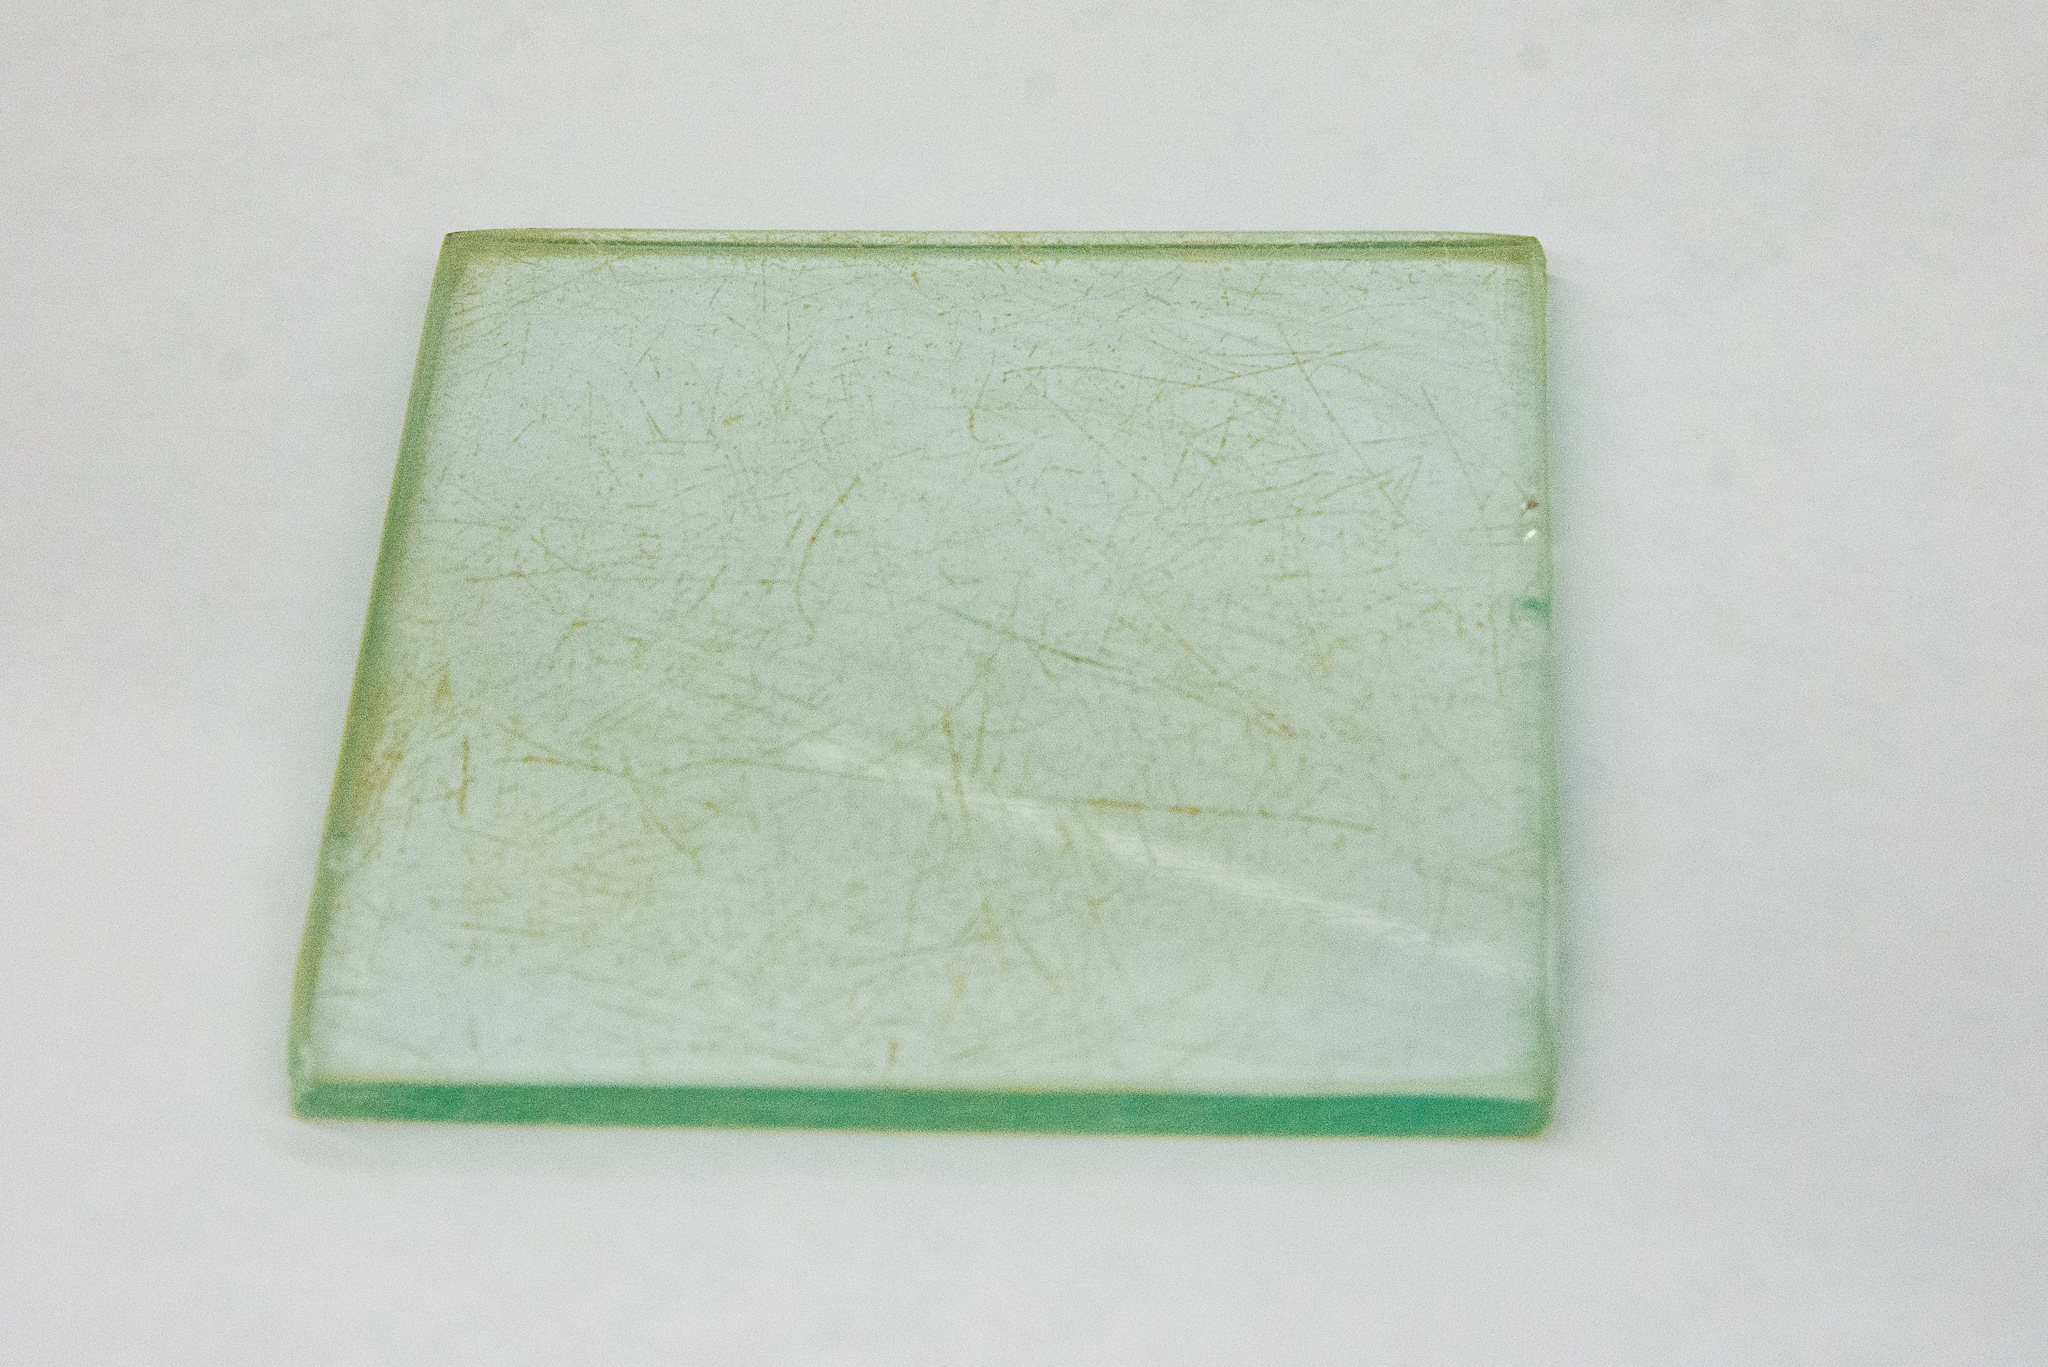
\includegraphics[width=0.7\textwidth]{GEO_5847.jpg}
    \caption{Example of the glass plate that will be used on top of the glass jar.}
    \label{fig:glassplate}
\end{figure}

Even though we will be calculating relative densities, which requires some known volumes, all of our measurements will be done on a weight-basis (i.e. all calculations are done using weights, not volumes). We are going to be recording a variety of weights\footnote{For this laboratory exercise, the terms ``weight'' and ``mass'' are used interchangeably. Since the materials being measured are not moving and we assume the gravitational force exerted on them is constant, we can safely make this assumption. Additionally, we are not calculating the force exerted by the materials. In other parts of this course, we will distinguish between weight and mass using gravity.} and it is important to prepare a worksheet prior to lab to aid in collecting the necessary data.

To aid us in creating a worksheet, let's look at ASTM C128 and see what is needed for the equations outlined in \S 10.0. An interactive PDF version of the ASTM standard is provided for you on Blackboard that will highlight some of the important measurements we will need to collect. Additionally, an example data collection worksheet is shown in Appendix A. It is important to note that the example worksheet assumes you obtained an SSD sample of exactly 500 grams! Be sure to use the numbers you obtained! There is also a fair amount of extraneous information since this is an actual form used by the North Dakota DOT. Additionally, note the use of deprecated terminology!

\subsubsection*{Preparation Checklist}
\begin{itemize}
    \item Obtain pan with aggregate sample
    \item Obtain pycnometer (i.e. pickle jar with glass plate)
    \item Prepare worksheet to record measurements (do this before lab)
\end{itemize}

\subsubsection{Execution}
We are now ready to execute the procedures outlined in ASTM C128. The first step is to calibrate the pycnometer. We are going to measure the volume of the fine aggregate sample by measuring how much water it displaces out of the pycnometer. We first need to determine the volume of the pycnometer by filling it completely with water. Once you have filled the container to the top, carefully slide the glass plate across the top to remove all air bubbles. It is very important that you slide the glass plate from one side to the other and not simply drop the plate from above. After you have confirmed the glass plate is fully over the mouth of the container and there are no air bubbles underneath the glass, dry off the container from any water that spilled out. Record the weight of the entire apparatus (i.e. container, water, and glass plate). This measurement is one of the values you need to calculate the relative densities.

The second step is to start the drying process of the fine aggregates. This is the hardest part of the process as it requires patience and experience to know when you are close to the SSD condition. You are looking for a state in which the sand just starts to become dry on the surface. One of the methods we can more quantitatively check for this is to compact a sample in a cone. If the sample collapses once the cone is removed, we have achieved SSD. If the sample stands up like a sand castle, we are still too wet. Another method is to use brown paper towels and tamp the sample. If no water is absorbed by the towel, it is likely at SSD. In order to speed up the process a little, you will just stir the sample for a short period and observe if it is too wet (sand castle stays up) or too dry (sand castle completely collapses). Once you have achieved SSD\footnote{In reality you will not achieve SSD, but something near it}, you will need to weigh out about 200 grams of the sample. Record the exact weight you weighed out.

You will then add the weighed sample of SSD aggregate to the pycnometer\footnote{Be sure to dump out about half of the water from the prior calibration process so you don't overflow the container}. Slowly add water to the pycnometer to begin filling it up again. As you fill up the pycnometer, carefully swish it around to dislodge any air bubbles that are trapped on or in the aggregate particles. Once you fill the pycnometer to the top, slide the glass plate across the mouth in the same fashion as the calibration steps. Dry off the container from any water that might have spilled and weigh the entire apparatus.

Finally, carefully remove the glass plate and pour out the water without loosing aggregate particles. Once you have dumped some of the water, dump the remaining water and aggregate sample into an oven pan. The sample will be oven dried for at least 24 hours and you will be provided with the weight of the oven dried aggregate. Be sure to note the label of the oven pan you dumped your sample into. Your results will only be identified through this label.

\subsubsection*{Execution Checklist}
\begin{itemize}
    \item Obtain weight of pycnometer filled with only water
    \item Obtain weight of SSD aggregate sample
    \item Obtain weight of pycnometer filled with water and aggregate sample
\end{itemize}

\subsubsection{Analysis}
The analysis portion for this laboratory exercise is straightforward. You will calculate the following values according to ASTM C128 \S 10:
\begin{itemize}
    \item Oven Dry Relative Density
    \item SSD Relative Density
    \item Apparent Relative Density
    \item Absorption
\end{itemize}

Every engineer should have some idea of the expected range of values to obtain through this test. The aggregate being characterized is ``typical'' and there is nothing special about it (e.g. lightweight, steel slag, etc). For normalweight aggregate, we should expect the relative density values to all be within 2.30 and 2.70. The apparent relative density can sometimes go up to 2.90. Absorption is typically between 1.0\% and 5.0\%. If your values are not in this range, you did something wrong. Check your calculations and if there is nothing wrong with those, it is likely you measured a weight incorrectly or lost some material along the way. That is okay, but you have to note that and provide a very brief explanation of where you think the error lies. Simply reporting a wrong number with no explanation will result in grade deductions.

There is another quick check we can do on the numbers. By definition, the oven dry relative density must be less than the SSD relative density. The SSD relative density must be less than the apparent relative density. It is physically impossible to have any other arrangement! If your numbers do not order correctly, you have a mistake somewhere that you need to correct and/or note in your datasheet.

Pay careful attention to the number of decimal places you are allowed to report your values to. Just because your calculator or Excel gives you ten decimal places does not mean that is appropriate to report. Fortunately, you do not have to worry about significant figures as most ASTM standards explicitly state the number of decimal places to use. This information is found in \S11.

\subsubsection*{Analysis Checklist}
\begin{itemize}
    \item Calculate the requested relative density and absorption capacity values
\end{itemize}

\subsection{Summary}
We have successfully planned, executed, and analyzed the results of a relative density characterization of a fine aggregate sample. This process is relatively straightforward but can be tricky getting to an exact SSD state. One important thing you should take away from this exercise is how we used weights and water displacements to calculate volumes to get a relative density value. This idea will be used for coarse aggregate testing in the next section.

\newpage
\section{Coarse Aggregates}
\label{sec:intro}
\normalsize 
There are several definitions for what constitutes a coarse aggregate. A geotechnical application may consider coarse aggregate to be anything larger than the \#4 sieve while an asphalt concrete application may consider coarse aggregate to be anything larger than 0.5 inches. However, let's look back at ASTM C125 to see what the definition of a coarse aggregate is:

\begin{letter}
(1) aggregate predominantly retained on the 4.75-mm (No. 4) sieve; or (2) that portion of an aggregate retained on the 4.75-mm (No. 4) sieve.
\end{letter}

We will use this definition for our laboratory exercise. Just like fine aggregates, the naming conventions that are used for coarse aggregate in ASTM specifications is shown in Table \ref{tab:ASTMname} along with their deprecated terms. We will continue to use the ``official'' terminology as outlined in the ASTM specifications.


\subsection{Objectives}
\label{ssec:headingscap}
At the completion of this lab exercise section, you will have satisfied the following objectives:
\begin{enumerate}
    \item Perform saturated-surface-dry (SSD) relative density measurement on a coarse aggregate
    \item Prepare coarse aggregate sample for oven-dry relative density measurement
    \item Perform calculations necessary to determine the relative density properties of a coarse aggregate
    \item Perform calculations necessary to determine the absorption capacity of a coarse aggregate
\end{enumerate}

\subsection{Learning Outcomes}
At the completion of this lab exercise, you should be able to:
\begin{itemize}
    \item understand what saturated-surface-dry and oven-dry conditions are for a coarse aggregate
    \item perform calculations necessary to characterize the relative density and absorption capacity of a coarse aggregate
    \item understand the appropriate range of possible values for relative density and absorption capacity for coarse aggregates
    \item present calculated values in a useful and professional manner
\end{itemize}

\pagebreak
\subsection{Procedure}
The coarse aggregate characterization procedure is divided into three parts: preparation, execution, and analysis. Given the importance placed on weight (mass) measurements, it is critical to keep detailed notes and follow steps carefully and accurately. There are a number of measurements that will be taken and it is easy to get the values mixed up. It may even help you to take a picture of the scale with the material on it for each step so you have a visual record of the weight and what was actually weighed.

Compared to the fine aggregate measurements, the coarse aggregate measurements are much simpler and faster. You will obtain a sample of coarse aggregate and then begin to dry them off with paper towels. Once the sample has reached SSD conditions, you will weigh out a sample. Then you will obtain the buoyant weight of the sample and finally oven dry the sample and obtain the oven-dry weight.

\subsubsection{Preparation}
For the coarse aggregate characterization, you will need your saturated sample and paper towels. Even though we will be calculating relative densities, which requires some known volumes, all of our measurements will be done on a weight-basis (i.e. all calculations are done using weights, not volumes). We are going to be recording a variety of weights and it is important to prepare a worksheet prior to lab to aid in collecting the necessary data.

To aid us in creating a worksheet, let's look at ASTM C127 and see what is needed for the equations outlined in \S 9.0. An interactive PDF version of the ASTM standard is provided for you on Blackboard that will highlight some of the important measurements we will need to collect. Additionally, an example data collection worksheet is shown in Appendix B.

\subsubsection*{Preparation Checklist}
\begin{itemize}
    \item Obtain saturated coarse aggregate sample
    \item Obtain damp towel
    \item Prepare worksheet to record measurements (do this prior to lab)
\end{itemize}

\subsubsection{Execution}
We are now ready to execute the procedures outlined in ASTM C127. Begin wiping your sample with the paper towels to remove the surface water. Keep doing so until there is no film of water remaining on the surface. You want the aggregates to lose their shine.

Immediately take a portion of the sample and weigh it on the scale. Your sample weight should be about 200 grams\footnote{Yes, this does deviate from the standard, a lot, but is done to accommodate the large number of samples that will be in the oven.}. Once you have the SSD weight, place the same sample in the wire mesh cage suspended under the scale (Fig. \ref{fig:cage}). Take care to prevent the cage from spinning excessively. Once the measurement has stabilized, record this buoyant weight (i.e. weight of sample in water).

\begin{figure}[H]
    \centering
    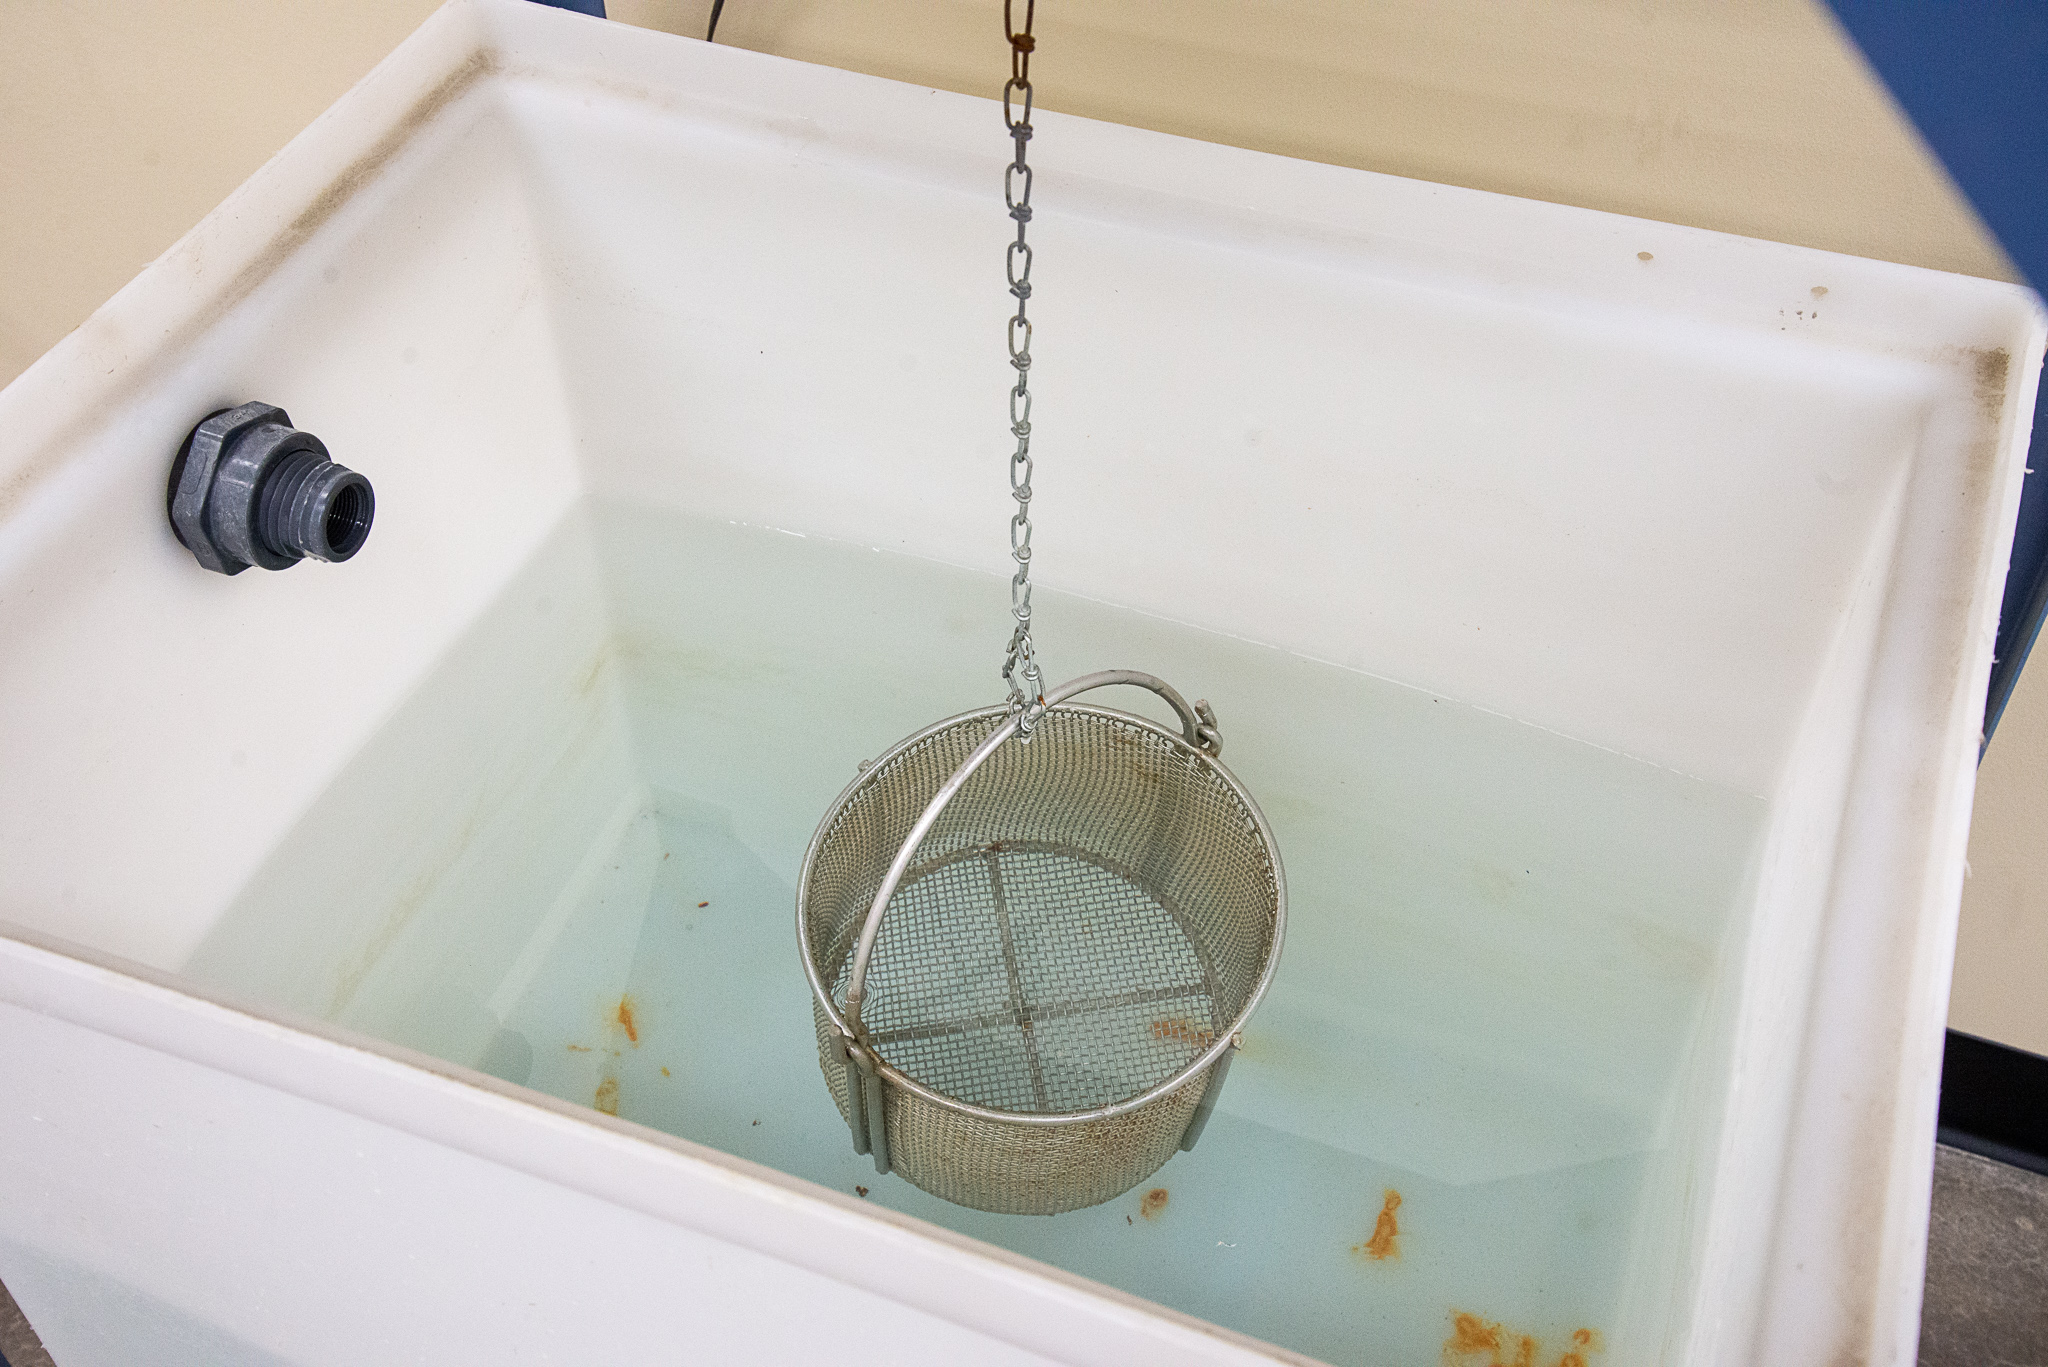
\includegraphics[width=0.7\textwidth]{GEO_5852.jpg}
    \caption{Suspended wire mesh cage hanging from a scale in a container of water. Always ensure the cage is as motionless as possible to get accurate results.}
    \label{fig:cage}
\end{figure}

Finally, remove the sample from the cage, ensuring you remove every single particle. Place in a container so that the sample can be oven-dried. The sample will be oven dried for at least 24 hours and you will be provided with the weight of the oven dried aggregate. Be sure to note the container label so that you can later identify your sample.

\subsubsection*{Execution Checklist}
\begin{itemize}
    \item Obtain weight of SSD sample
    \item Obtain weight of buoyant sample
\end{itemize}

\subsubsection{Analysis}
The analysis portion for this laboratory exercise is straightforward. You will calculate the following values according to ASTM C127 \S 9:
\begin{itemize}
    \item Oven Dry Relative Density
    \item SSD Relative Density
    \item Apparent Relative Density
    \item Absorption
\end{itemize}

You may be surprised to learn that we are expecting the same ranges of values as we did with the fine aggregate! Additionally, the ordering of oven dry, SSD, and apparent relative densities is the same as those described for the fine aggregate.

Pay careful attention to the number of decimal places you are allowed to report your values to. Just because your calculator or Excel gives you ten decimal places does not mean that is appropriate to report. Fortunately, you do not have to worry about significant figures as most ASTM standards explicitly state the number of decimal places to use. This information is found in \S10.

\subsubsection*{Analysis Checklist}
\begin{itemize}
    \item Calculate the requested relative density and absorption capacity values
\end{itemize}

\subsection{Summary}
We have successfully planned, executed, and analyzed the results of a relative density characterization of a coarse aggregate sample. This process is very straightforward but very important for future calculations. One important thing you should take away from this exercise is how we used weights and water displacements to calculate volumes to get a relative density value. 
\pagebreak
\section{Deliverables}
For this laboratory exercise, you will need to submit two datasheets following the general format of the example worksheets in Appendix A and B. Some of the details listed in the example, such as ``Location'' and ``Owner'' are not necessary for you to include. Create a separate page(s) for each aggregate source and at a minimum include:
\begin{itemize}
    \item The weights used in the equations from ASTM C127 and C128
    \item Method for determining SSD (fine aggregate)
\end{itemize}

A large part of this exercise is professional formatting. You will likely spend more time making the page(s) look good than performing the actual calculations and this is okay! Professional engineers will typically use software specifically designed to make nice sheets. However, there are still some firms and engineers that do it manually. Most of the time the entire page is created in MS Excel due to the insane number of rows and columns needed. Here are some DOs and DON'Ts to help guide you in making a professional submission:

\begin{itemize}
    \item DO be consistent with decimal places and where applicable, follow the ASTM rules for number of decimal places
    \item DO indicate units properly
    \item DON'T use a font size smaller than 10pt
    \item DON'T use shading (i.e. shading alternating rows)
\end{itemize}

%\section*{References}
%\addcontentsline{toc}{section}{References}
%\bibliographystyle{techpubs}
%\bibliography{References}

%%%%%%%%%%%%%%%%%%%%%%%%%%%%%%%%%%%%%%%%%%%%%%%%%%%%%%%%%%%%%%%%%%%%
%   Please use the techpubs BibTeX style when compiling bibliography, or follow the instructions on tinyurl.com/techpubsnist to format your .bib / .bbl file appropriately.
%%%%%%%%%%%%%%%%%%%%%%%%%%%%%%%%%%%%%%%%%%%%%%%%%%%%%%%%%%%%%%%%%%%%
\pagebreak

\section*{Appendix A: Example Fine Aggregate Worksheet}
\label{AppendixA}
\addcontentsline{toc}{section}{Appendix A: Example Fine Aggregate Worksheet}
\begin{center}
    \includegraphics[width=1\linewidth]{NDDOT_Fine_Agg.eps}
\end{center}

\pagebreak

\section*{Appendix B: Example Coarse Aggregate Worksheet}
\label{AppendixA}
\addcontentsline{toc}{section}{Appendix B: Example Coarse Aggregate Worksheet}
\begin{center}
    \includegraphics[width=1\linewidth]{NDDOT_Coare_Agg.eps}
\end{center}

%\pagebreak
%\section*{Appendix B: Change Log}
%\addcontentsline{toc}{section}{Appendix B: Change Log}
%This document was originally created on April 9, 2020. Any changes will be documented in this appendix.

\end{document}
%%%%%%%%%%%%%%%%%%%%%%%%%%%%%%%%%%%%%%%%%%%%%%%%%%%%%%%%%%%%%%%%%%%%
%   When referring to references in the text parenthetically, 
%	use the form “[1].” For example, “As Jones and Smith have shown [1];”
%	 however, when a reference is referred to non-parenthetically, use the form 
%	“. . . Ref. [1] . . .” (except at the beginning of a sentence where
%	“Reference [1] . . .” is the correct form).
%%%%%%%%%%%%%%%%%%%%%%%%%%%%%%%%%%%%%%%%%%%%%%%%%%%%%%%%%%%%%%%%%%%%

%%%%%%%%%%%%%%%%%%%%%%%%%%%%%%%%%%%%%%%%%%%%%%%%%%%%%%%%%%%%%%%%%%%%
%   Section references are “Sec. X”.
% 	“Section X” is used at beginning of sentence. 
%%%%%%%%%%%%%%%%%%%%%%%%%%%%%%%%%%%%%%%%%%%%%%%%%%%%%%%%%%%%%%%%%%%%

%%%%%%%%%%%%%%%%%%%%%%%%%%%%%%%%%%%%%%%%%%%%%%%%%%%%%%%%%%%%%%%%%%%%
%   Equation references are “Eq. (X)”.
% 	“Equation (1) is used at beginning of sentence.
%	Equations are numbered (#) on the right, per the standard LaTeX format
%%%%%%%%%%%%%%%%%%%%%%%%%%%%%%%%%%%%%%%%%%%%%%%%%%%%%%%%%%%%%%%%%%%%

%%%%%%%%%%%%%%%%%%%%%%%%%%%%%%%%%%%%%%%%%%%%%%%%%%%%%%%%%%%%%%%%%%%%
%   Tables should appear after they are mentioned in the text. 
%	Superscripted letters (a, b, c, etc.) should be used for table footnotes.
%%%%%%%%%%%%%%%%%%%%%%%%%%%%%%%%%%%%%%%%%%%%%%%%%%%%%%%%%%%%%%%%%%%%

%%%%%%%%%%%%%%%%%%%%%%%%%%%%%%%%%%%%%%%%%%%%%%%%%%%%%%%%%%%%%%%%%%%%
%   Figure references are “Fig. X”.
% 	“Figure X” is used at beginning of sentence. 
% 	Figures should appear after they are mentioned in the text.
%	Figures must have embedded alternate text or “alt text” in order 
%	to comply with Section 508 accessibility standards. 
%%%%%%%%%%%%%%%%%%%%%%%%%%%%%%%%%%%%%%%%%%%%%%%%%%%%%%%%%%%%%%%%%%%%